% %% %%%%%%%%%%%%%%%%%%%%%%%%%%%%%%%%%%%%%%%%%%%%%%%%%%%%%%%%%%
% practica.tex
%
% Author:  Mauricio Matamoros
% License: MIT
%
% %% %%%%%%%%%%%%%%%%%%%%%%%%%%%%%%%%%%%%%%%%%%%%%%%%%%%%%%%%%%

% CHKTEX-FILE 1
% CHKTEX-FILE 46
\documentclass[letterpaper,10.5pt]{article}
% %% %%%%%%%%%%%%%%%%%%%%%%%%%%%%%%%%%%%%%%%%%%%%%%%%%%%%%%%%%
%
% packages.tex
%
%  Author: Mauricio Matamoros
%  Date:   2020.02.28
%
%  Contiene la lista de paquetes requeridos para generar
%  el archivo-reporte de las prácticas de laboratorio
%
% %% %%%%%%%%%%%%%%%%%%%%%%%%%%%%%%%%%%%%%%%%%%%%%%%%%%%%%%%%%
% Archivo principal de LaTeX
%!TEX root = ../reporte.tex

\usepackage[utf8]{inputenc}                  % Soporte para utf8
\usepackage[T1]{fontenc}                     % Soporte extendido de caracteres unicode
\usepackage[english,spanish,mexico]{babel}   % Define el idioma del documento a español (México) con soporte para inglés
% Standard packages
\usepackage{float}                           % Imágenes flotantes en el documento
\usepackage{ifthen}                          % Soporte if-then en macros
\usepackage{xspace}                          % Soporte de autoespaciado en macros
\usepackage{xstring}                         % Operaciones con cadenas en macros
\usepackage{wrapfig}                         % Permite colocar texto al rededor de figuras y otros flotantes
\usepackage{booktabs}                        % Embellece tablas
\usepackage{csquotes}                        % Entrecomillado automático y manejo de citas textuales
\usepackage{fancyhdr}                        % Permite reconfigurar encabezado y pie de página
\usepackage{fancyvrb}                        % Define estilos para entornos Verbatim
\usepackage{geometry}                        % Permite reconfigurar la geometría del documento
\usepackage{graphicx}                        % Permite insertar imágenes en varios formatos
\usepackage{lastpage}                        % Referencia a la última página del documento
\usepackage{listings}                        % Define estilos para entornos de código de programación (sintaxis)
\usepackage{multicol}                        % Manejo de texto en varias columnas
\usepackage{tabularx}                        % Tablas con ancho de columna variable
\usepackage{algorithm}                       % Entorno para escribir algoritmos
\usepackage{algpseudocode}                   % Entorno para escribir algoritmos en pseudocódigo
\usepackage[justification=centering]{subcaption} % Permite imágenes en viñetas
\usepackage[all]{nowidow}                    % Control de viudas y huérfanas
\usepackage[inline]{enumitem}                % Añade opciones de configuración a listas
\usepackage[usenames,dvipsnames]{xcolor}     % Permite el uso de colores en el documento
% Referencing
\usepackage{varioref}                        % Gestión de referencias variables
\usepackage{hyperref}                        % Gestión de referencias e hipervínculos
\usepackage[noabbrev,nameinlink,spanish]{cleveref} % Gestión de referencias cruzadas inteligentes con hipervínculos
\usepackage[square, comma, numbers, sort&compress]{natbib} % Gestión de referencias bibliográficas


\newcommand{\lpar}{(}\newcommand{\rpar}{)} %CHKTEX 9
\newcommand{\IIC}{I\textsuperscript{2}C\xspace}
\newcommand{\GND}{\textsc{Gnd}\xspace}
\newcommand{\VCC}{\textsc{Vcc}\xspace}
\newcommand{\VDD}{\textsc{Vdd}\xspace}
\newcommand{\textbi}[1]{\textbf{\textit{#1}}}
\newcommand{\degreesC}[1]{%
	#1\textsuperscript{o}C\xspace{}%
}
\newcommand{\degreesF}[1]{%
	#1\textsuperscript{o}F\xspace{}%
}

% \newcommand{\VCC}{V\textsubscript{CC}\xspace{}}
% \newcommand{\GND}{\textsc{Gnd}\xspace{}}
% CHKTEX-FILE 26
% CHKTEX-FILE 36

\tcbuselibrary{most}
% \tcbuselibrary{listings,breakable}
% \usetikzlibrary{shadings,shadows}
% \usetikzlibrary{decorations.pathmorphing}
% \usetikzlibrary{patterns}
% \usetikzlibrary{spy}
% \usetikzlibrary{arrows.meta}

\newtcolorbox{importantbox}[1]{%
	enhanced,
	colback=red!5!white,%
	colframe=red!75!black,%
	fonttitle=\bfseries,%
	center title,
	title={#1},%
	drop fuzzy shadow
}


\newtcolorbox{greenbox}[1]{%
	enhanced,
	colback=Green!5!white,%
	colframe=Green!75!black,%
	fonttitle=\bfseries,%
	center title,
	title={#1},%
	drop fuzzy shadow
}

\newtcolorbox{marker}[1][]{%
	enhanced,
	before skip=2mm,after skip=3mm,
	boxrule=0.4pt,left=5mm,right=2mm,top=1mm,bottom=1mm,
	colback=yellow!50,
	colframe=yellow!20!black,
	sharp corners,rounded corners=southeast,arc is angular,arc=3mm,
%	underlay={%
%		\path[fill=tcbcolback!80!black] ([yshift=3mm]interior.south east)--++(-0.4,-0.1)--++(0.1,-0.2);
%		\path[draw=tcbcolframe,shorten <=-0.05mm,shorten >=-0.05mm] ([yshift=3mm]interior.south east)--++(-0.4,-0.1)--++(0.1,-0.2);
%		\path[fill=yellow!50!black,draw=none] (interior.south west) rectangle node[white]{\Huge\bfseries !} ([xshift=4mm]interior.north west);
%	},
	drop fuzzy shadow,#1
}

%CHKTEX-FILE 1
%CHKTEX-FILE 7
%CHKTEX-FILE 9
% Default fixed font does not support bold face
\DeclareFixedFont{\ttb}{T1}{txtt}{bx}{n}{8} % for bold
\DeclareFixedFont{\ttm}{T1}{txtt}{m}{n}{8}  % for normal

% Custom colors
\usepackage{color}
\definecolor{keywordsColor}{rgb}{0,0,0.5}
\definecolor{customColor}{rgb}{0.6,0,0}
\definecolor{stringColor}{rgb}{0,0.5,0}

% Code highlighting python
\renewcommand{\ttdefault}{pcr}
\lstset{
	language=Python,                              % the language of the code (can be overrided per snippet)
	backgroundcolor=\color{white},                % choose the background color
	basicstyle=\footnotesize\ttfamily,            % the size of the fonts that are used for the code
	breakatwhitespace=false,                      % sets if automatic breaks should only happen at whitespace
	breaklines=true,                              % sets automatic line breaking
	captionpos=t,                                 % sets the caption-position to bottom
	commentstyle=\color{gray},                    % comment style
	deletekeywords={},                            % if you want to delete keywords from the given language
%	escapeinside={\%*}{*)},                       % if you want to add LaTeX within your code
	extendedchars=true,                           % lets you use non-ASCII characters; for 8-bits encodings only, does not work with UTF-8
	frame=tb,                                     % adds a frame around the code
	keepspaces=true,                              % keeps spaces in text, useful for keeping indentation of code (possibly needs columns=flexible)
	keywordstyle=\color{keywordsColor}\bfseries,  % keyword style
	numbers=left,                                 % where to put the line-numbers; possible values are (none, left, right)
	numbersep=5pt,                                % how far the line-numbers are from the code
	numberstyle=\tiny\color{gray},                % the style that is used for the line-numbers
	rulecolor=\color{black},                      % if not set, the frame-color may be changed on line-breaks within not-black text (e.g. comments (green here))
	showspaces=false,                             % show spaces everywhere adding particular underscores; it overrides 'showstringspaces'
	showstringspaces=false,                       % underline spaces within strings only
	showtabs=false,                               % show tabs within strings adding particular underscores
	stepnumber=1,                                 % the step between two line-numbers. If it's 1, each line will be numbered
	stringstyle=\color{stringColor},              % string literal style
	tabsize=2,                                    % sets default tabsize to 2 spaces
	title=\lstname,                               % show the filename of files included with \lstinputlisting; also try caption instead of title
	columns=fixed,                                % Using fixed column width (for e.g. nice alignment)
	otherkeywords={self},                         % if you want to add more keywords to the set
	emphstyle=\color{customColor}\bfseries,       % Custom highlighting style
	emph={__init__,__main__,True,False,None},     % Custom highlighting keywords
	xleftmargin=1cm,                              % Left margin
	xrightmargin=1cm,                             % Right margin
	% Unicode compatibility
	inputencoding=utf8,
	literate={%
	            {Á}{{\'a}}1 {É}{{\'E}}1 {Í}{{\'I}}1 {Ó}{{\'O}}1 {Ú}{{\'U}}1%
	            {á}{{\'a}}1 {é}{{\'e}}1 {í}{{\'i}}1 {ó}{{\'o}}1 {ú}{{\'u}}1%
	            {À}{{\`A}}1 {È}{{\'E}}1 {Ì}{{\`I}}1 {Ò}{{\`O}}1 {Ù}{{\`U}}1%
	            {à}{{\`a}}1 {è}{{\`e}}1 {ì}{{\`i}}1 {ò}{{\`o}}1 {ù}{{\`u}}1%
	            {Ä}{{\"A}}1 {Ë}{{\"E}}1 {Ï}{{\"I}}1 {Ö}{{\"O}}1 {Ü}{{\"U}}1%
	            {ä}{{\"a}}1 {ë}{{\"e}}1 {ï}{{\"i}}1 {ö}{{\"o}}1 {ü}{{\"u}}1%
	            {Â}{{\^A}}1 {Ê}{{\^E}}1 {Î}{{\^I}}1 {Ô}{{\^O}}1 {Û}{{\^U}}1%
	            {â}{{\^a}}1 {ê}{{\^e}}1 {î}{{\^i}}1 {ô}{{\^o}}1 {û}{{\^u}}1% CHKTEX 19
	            {Ã}{{\~a}}1 {Ẽ}{{\~E}}1 {Ĩ}{{\~I}}1 {Õ}{{\~O}}1 {Ũ}{{\~U}}1 {Ñ}{{\~N}}1%
	            {ã}{{\~a}}1 {ẽ}{{\~e}}1 {ĩ}{{\~i}}1 {õ}{{\~o}}1 {ũ}{{\~u}}1 {ñ}{{\~n}}1%
	            {œ}{{\oe}}1 {Œ}{{\OE}}1 {æ}{{\ae}}1 {Æ}{{\AE}}1 {ß}{{\ss}}1%
	            {ç}{{\c c}}1 {Ç}{{\c C}}1 {ø}{{\o}}1 {å}{{\r a}}1 {Å}{{\r A}}1%
	            {€}{{\EUR}}1 {£}{{\pounds}}1 {×}{{\(\times\)}}1% CHKTEX 21
	            {°}{{\textsuperscript{o}}}1%
	            {¹}{{\textsuperscript{1}}}1%
	            {²}{{\textsuperscript{2}}}1%
	            {³}{{\textsuperscript{3}}}1%
	            {⁴}{{\textsuperscript{4}}}1% CHKTEX 19
	            {⁵}{{\textsuperscript{5}}}1% CHKTEX 19
	            {⁶}{{\textsuperscript{6}}}1% CHKTEX 19
	            {⁷}{{\textsuperscript{7}}}1% CHKTEX 19
	            {⁸}{{\textsuperscript{8}}}1% CHKTEX 19
	            {⁹}{{\textsuperscript{9}}}1% CHKTEX 19
	            {⁰}{{\textsuperscript{0}}}1% CHKTEX 19
%	            {A}{{\textAlpha}}1
	            {α}{{\textalpha}}1%
%	            {B}{{\textBeta}}1
	            {β}{{\textbeta}}1%
	            {Γ}{{\textGamma}}1
	            {γ}{{\textgamma}}1%
	            {Δ}{{\textDelta}}1
	            {δ}{{\textdelta}}1% CHKTEX 19
%	            {E}{{\textEpsilon}}1
	            {ϵ}{{\textepsilon}}1%
%	            {Z}{{\textZeta}}1
	            {ζ}{{\textzeta}}1%
%	            {H}{{\textEta}}1
	            {η}{{\texteta}}1%
	            {Θ}{{\textTheta}}1
	            {θ}{{\texttheta}}1%
%	            {I}{{\textIota}}1
	            {ι}{{\textiota}}1%
%	            {K}{{\textKappa}}1
	            {κ}{{\textkappa}}1%
	            {Λ}{{\textLambda}}1
	            {λ}{{\textlambda}}1%
%	            {M}{{\textMu}}1
	            {μ}{{\textmu}}1%
%	            {N}{{\textNu}}1
	            {ν}{{\textnu}}1%
	            {Ξ}{{\textXi}}1
	            {ξ}{{\textxi}}1%
%	            {O}{{\textOmikron}}1
%	            {o}{{\textomikron}}1%
	            {Π}{{\textPi}}1
	            {π}{{\textpi}}1%
%	            {P}{{\textRho}}1
	            {ρ}{{\textrho}}1%
	            {Σ}{{\textSigma}}1
	            {σ}{{\textsigma}}1%
%	            {T}{{\textTau}}1
	            {τ}{{\texttau}}1%
	            {ϒ}{{\textUpsilon}}1
	            {υ}{{\textupsilon}}1%
	            {Φ}{{\textPhi}}1
	            {ϕ}{{\textphi}}1%
%	            {X}{{\textChi}}1
	            {χ}{{\textchi}}1%
	            {Ψ}{{\textPsi}}1
	            {ψ}{{\textpsi}}1%
	            {Ω}{{\textOmega}}1
	            {ω}{{\textomega}}1%
	            {ζ}{{\varsigma}}1%
%	            {}{{\straightphi}}1%
%	            {}{{\scripttheta}}1%
%	            {}{{\straighttheta}}1%
%	            {}{{\straightepsilon}}1%
	         },
}

\lstdefinestyle{c_with_comments}%
{
	language     = c,
	morecomment  = [l]{//},
	morecomment  = [s]{/*}{*/},
	breaklines,
}

\lstdefinestyle{c_without_comments}{%
	style        = c_with_comments,
	% numbers      = none,
	% keepspaces   = false,
	morecomment  = [l][\nullfont]{//},
	morecomment  = [is]{//}{\^^M},
	morecomment  = [is]{/*}{*/},
	emptylines   = *1,
}

\lstdefinestyle{py_without_comments}{%
	language     = python,
	morecomment  = [l][\nullfont]{\#},
	% morecomment  = [il]{\#},
	% morecomment  = [is]{\#}{\^^M},
	emptylines   = *1,
}

\lstdefinestyle{py_without_doclines}{%
	morecomment  = [is]{'''}{'''},%CHKTEX 23
	morecomment  = [is]{"""}{"""},%CHKTEX 18
	morecomment  = [is]{\#'''}{'''},%CHKTEX 23
	morecomment  = [is]{\#"""}{"""},%CHKTEX 18
}

\lstdefinelanguage{conf}
{
	basicstyle=\ttfamily\small,
	columns=fullflexible,
	morecomment=[s][\color{Orchid}\bfseries]{[}{]},
	morecomment=[l]{\#},
	morecomment=[l]{;},
	commentstyle=\color{gray}\ttfamily,
	% morekeywords={},
	% otherkeywords={=,:},
	% keywordstyle={\color{Green}\bfseries}
}

% \captionsetup[lstlisting]{font={small,tt}}
\captionsetup[lstlisting]{%
	font={small},
}



\DefineVerbatimEnvironment{Verbatim}{Verbatim}{%
	fontsize=\footnotesize,%
	frame=leftline,%
	framesep=2em,    % separation between frame and text
}

\RecustomVerbatimCommand{\VerbatimInput}{VerbatimInput}{%
	fontsize=\footnotesize,
%	frame=lines,            % top and bottom rule only
	frame=leftline,         % left rule only
	numbers=left,           % Line numbers on the left
	numbersep=0.25em,       % Gap between numbers and verbatim lines
	xleftmargin=4em,        % Indentation to add at the start of each line
	xrightmargin=4em,       % Right margin to add after each line
	framesep=0.5em,         % separation between frame and text
	rulecolor=\color{Gray}, % Color of the lines
	labelposition=topline,  %
	samepage=false,         % When true, prevents verbatim environment from
	                        % being broken between pages
%	commandchars=\|\(\),    % escape character and argument delimiters for
	                        % commands within the verbatim
%	commentchar=*           % comment character
}


% CHKTEX-FILE 1
% CHKTEX-FILE 13
% CHKTEX-FILE 18
% CHKTEX-FILE 35
\documentclass[letterpaper,12pt,twocolumn]{article}
% Input encodign

% %% %%%%%%%%%%%%%%%%%%%%%%%%%%%%%%%%%%%%%%%%%%%%%%%%%%%%%%%%%
%
% packages.tex
%
%  Author: Mauricio Matamoros
%  Date:   2020.02.28
%
%  Contiene la lista de paquetes requeridos para generar
%  el archivo-reporte de las prácticas de laboratorio
%
% %% %%%%%%%%%%%%%%%%%%%%%%%%%%%%%%%%%%%%%%%%%%%%%%%%%%%%%%%%%
% Archivo principal de LaTeX
%!TEX root = ../reporte.tex

\usepackage[utf8]{inputenc}                  % Soporte para utf8
\usepackage[T1]{fontenc}                     % Soporte extendido de caracteres unicode
\usepackage[english,spanish,mexico]{babel}   % Define el idioma del documento a español (México) con soporte para inglés
% Standard packages
\usepackage{float}                           % Imágenes flotantes en el documento
\usepackage{ifthen}                          % Soporte if-then en macros
\usepackage{xspace}                          % Soporte de autoespaciado en macros
\usepackage{xstring}                         % Operaciones con cadenas en macros
\usepackage{wrapfig}                         % Permite colocar texto al rededor de figuras y otros flotantes
\usepackage{booktabs}                        % Embellece tablas
\usepackage{csquotes}                        % Entrecomillado automático y manejo de citas textuales
\usepackage{fancyhdr}                        % Permite reconfigurar encabezado y pie de página
\usepackage{fancyvrb}                        % Define estilos para entornos Verbatim
\usepackage{geometry}                        % Permite reconfigurar la geometría del documento
\usepackage{graphicx}                        % Permite insertar imágenes en varios formatos
\usepackage{lastpage}                        % Referencia a la última página del documento
\usepackage{listings}                        % Define estilos para entornos de código de programación (sintaxis)
\usepackage{multicol}                        % Manejo de texto en varias columnas
\usepackage{tabularx}                        % Tablas con ancho de columna variable
\usepackage{algorithm}                       % Entorno para escribir algoritmos
\usepackage{algpseudocode}                   % Entorno para escribir algoritmos en pseudocódigo
\usepackage[justification=centering]{subcaption} % Permite imágenes en viñetas
\usepackage[all]{nowidow}                    % Control de viudas y huérfanas
\usepackage[inline]{enumitem}                % Añade opciones de configuración a listas
\usepackage[usenames,dvipsnames]{xcolor}     % Permite el uso de colores en el documento
% Referencing
\usepackage{varioref}                        % Gestión de referencias variables
\usepackage{hyperref}                        % Gestión de referencias e hipervínculos
\usepackage[noabbrev,nameinlink,spanish]{cleveref} % Gestión de referencias cruzadas inteligentes con hipervínculos
\usepackage[square, comma, numbers, sort&compress]{natbib} % Gestión de referencias bibliográficas


\newcommand{\lpar}{(}\newcommand{\rpar}{)} %CHKTEX 9
\newcommand{\IIC}{I\textsuperscript{2}C\xspace}
\newcommand{\GND}{\textsc{Gnd}\xspace}
\newcommand{\VCC}{\textsc{Vcc}\xspace}
\newcommand{\VDD}{\textsc{Vdd}\xspace}
\newcommand{\textbi}[1]{\textbf{\textit{#1}}}
\newcommand{\degreesC}[1]{%
	#1\textsuperscript{o}C\xspace{}%
}
\newcommand{\degreesF}[1]{%
	#1\textsuperscript{o}F\xspace{}%
}

% \newcommand{\VCC}{V\textsubscript{CC}\xspace{}}
% \newcommand{\GND}{\textsc{Gnd}\xspace{}}
% CHKTEX-FILE 1
% CHKTEX-FILE 13
% CHKTEX-FILE 18
% CHKTEX-FILE 35
\documentclass[letterpaper,12pt,twocolumn]{article}
% Input encodign

% %% %%%%%%%%%%%%%%%%%%%%%%%%%%%%%%%%%%%%%%%%%%%%%%%%%%%%%%%%%
%
% packages.tex
%
%  Author: Mauricio Matamoros
%  Date:   2020.02.28
%
%  Contiene la lista de paquetes requeridos para generar
%  el archivo-reporte de las prácticas de laboratorio
%
% %% %%%%%%%%%%%%%%%%%%%%%%%%%%%%%%%%%%%%%%%%%%%%%%%%%%%%%%%%%
% Archivo principal de LaTeX
%!TEX root = ../reporte.tex

\usepackage[utf8]{inputenc}                  % Soporte para utf8
\usepackage[T1]{fontenc}                     % Soporte extendido de caracteres unicode
\usepackage[english,spanish,mexico]{babel}   % Define el idioma del documento a español (México) con soporte para inglés
% Standard packages
\usepackage{float}                           % Imágenes flotantes en el documento
\usepackage{ifthen}                          % Soporte if-then en macros
\usepackage{xspace}                          % Soporte de autoespaciado en macros
\usepackage{xstring}                         % Operaciones con cadenas en macros
\usepackage{wrapfig}                         % Permite colocar texto al rededor de figuras y otros flotantes
\usepackage{booktabs}                        % Embellece tablas
\usepackage{csquotes}                        % Entrecomillado automático y manejo de citas textuales
\usepackage{fancyhdr}                        % Permite reconfigurar encabezado y pie de página
\usepackage{fancyvrb}                        % Define estilos para entornos Verbatim
\usepackage{geometry}                        % Permite reconfigurar la geometría del documento
\usepackage{graphicx}                        % Permite insertar imágenes en varios formatos
\usepackage{lastpage}                        % Referencia a la última página del documento
\usepackage{listings}                        % Define estilos para entornos de código de programación (sintaxis)
\usepackage{multicol}                        % Manejo de texto en varias columnas
\usepackage{tabularx}                        % Tablas con ancho de columna variable
\usepackage{algorithm}                       % Entorno para escribir algoritmos
\usepackage{algpseudocode}                   % Entorno para escribir algoritmos en pseudocódigo
\usepackage[justification=centering]{subcaption} % Permite imágenes en viñetas
\usepackage[all]{nowidow}                    % Control de viudas y huérfanas
\usepackage[inline]{enumitem}                % Añade opciones de configuración a listas
\usepackage[usenames,dvipsnames]{xcolor}     % Permite el uso de colores en el documento
% Referencing
\usepackage{varioref}                        % Gestión de referencias variables
\usepackage{hyperref}                        % Gestión de referencias e hipervínculos
\usepackage[noabbrev,nameinlink,spanish]{cleveref} % Gestión de referencias cruzadas inteligentes con hipervínculos
\usepackage[square, comma, numbers, sort&compress]{natbib} % Gestión de referencias bibliográficas


\newcommand{\lpar}{(}\newcommand{\rpar}{)} %CHKTEX 9
\newcommand{\IIC}{I\textsuperscript{2}C\xspace}
\newcommand{\GND}{\textsc{Gnd}\xspace}
\newcommand{\VCC}{\textsc{Vcc}\xspace}
\newcommand{\VDD}{\textsc{Vdd}\xspace}
\newcommand{\textbi}[1]{\textbf{\textit{#1}}}
\newcommand{\degreesC}[1]{%
	#1\textsuperscript{o}C\xspace{}%
}
\newcommand{\degreesF}[1]{%
	#1\textsuperscript{o}F\xspace{}%
}

% \newcommand{\VCC}{V\textsubscript{CC}\xspace{}}
% \newcommand{\GND}{\textsc{Gnd}\xspace{}}
% CHKTEX-FILE 1
% CHKTEX-FILE 13
% CHKTEX-FILE 18
% CHKTEX-FILE 35
\documentclass[letterpaper,12pt,twocolumn]{article}
% Input encodign

\input{setup/packages}
\input{setup/macros}
\input{setup/document}
\input{setup/listings}

\author{\footnotesize Autor: José Mauricio Matamoros de Maria y Campos}
\title{Especificación para reportes de lectura}
\date{}


% Document body
\begin{document}
\maketitle

\section*{Reportes de lectura}
El objetivo de las lecturas asignadas como tarea es fomentar en el alumno el hábito de la lectura, tanto de documentos técnicos como literarios, ya sean estos en español o en inglés, además de incrementar las habilidades de comprensión de lectura, concreción de ideas, síntesis y redacción de texto en prosa.

Leer es muy importante en el aprendizaje pues la mayor parte de lo que se aprende se hace por medio de la lectura.
Cuando se quiere aprender algo, lo primero que se hace es leer.

Cuando se lee un texto con fines de estudio se resaltan las ideas importantes, se resume, se separan las ideas principales y se formulan cuestionarios para mejor comprender el texto. Cuando se lee por entretenimiento (por ejemplo un cuento o una novela), el texto se analiza y se relacionan hechos y situaciones a fin de poder disfrutar de él.

Un reporte de lectura es un informe escrito acerca del texto que se leyó.
Este informe debe contener los siguientes datos:

\begin{itemize}[noitemsep]
	\item Título del texto y nombre del autor
	\item Tema o asunto que trata
	\item Resumen, síntesis o reseña del texto
	\item Análisis crítico del contenido del texto
	\item Opinión personal del contenido de la lectura
	\item Conclusiones de la lectura
\end{itemize}

En el caso de texto literario no se espera un resumen, síntesis o reseña del texto, sino que deberá comentarse sobre la temática del mismo y resaltar los puntos más importantes, dejando claras sus impresiones y comentarios sobre el texto.

Tome en cuenta que ni la síntesis ni los resúmenes implican copiar y pegar párrafos enteros del texto. Lo importante es distinguir las ideas principales, hacerlas propias y (salvo que sean definiciones), parafrasearlas, es decir,  expresarlas en sus propias palabras.

Pasos para elaborar un reporte de lectura
\begin{enumerate}[noitemsep]
	\item Lea atentamente el texto. Evite distractores como música fuerte, televisión, teléfono, etc.
	\item Anote los términos y palabras que no conozca o entienda e investigue su significado en un diccionario.
	\item Una vez aclarados los términos desconocidos y palabras nuevas, vuelva a leer el texto para comprenderlo mejor.
	\item En la segunda lectura subraye o marque las ideas principales del texto.
	%Procure no escribir en los libros, especialmente si no le pertenecen. Si desea hacer anotaciones, utilice un lápiz blando y escriba con suavidad, o de preferencia use fotocopias.
	\item Tome las ideas principales, abstraígalas, analícelas y sólo entonces redacte su escrito.
\end{enumerate}
\end{document}

%CHKTEX-FILE 1
%CHKTEX-FILE 7
%CHKTEX-FILE 9
% Default fixed font does not support bold face
\DeclareFixedFont{\ttb}{T1}{txtt}{bx}{n}{8} % for bold
\DeclareFixedFont{\ttm}{T1}{txtt}{m}{n}{8}  % for normal

% Custom colors
\usepackage{color}
\definecolor{keywordsColor}{rgb}{0,0,0.5}
\definecolor{customColor}{rgb}{0.6,0,0}
\definecolor{stringColor}{rgb}{0,0.5,0}

% Code highlighting python
\renewcommand{\ttdefault}{pcr}
\lstset{
	language=Python,                              % the language of the code (can be overrided per snippet)
	backgroundcolor=\color{white},                % choose the background color
	basicstyle=\footnotesize\ttfamily,            % the size of the fonts that are used for the code
	breakatwhitespace=false,                      % sets if automatic breaks should only happen at whitespace
	breaklines=true,                              % sets automatic line breaking
	captionpos=t,                                 % sets the caption-position to bottom
	commentstyle=\color{gray},                    % comment style
	deletekeywords={},                            % if you want to delete keywords from the given language
%	escapeinside={\%*}{*)},                       % if you want to add LaTeX within your code
	extendedchars=true,                           % lets you use non-ASCII characters; for 8-bits encodings only, does not work with UTF-8
	frame=tb,                                     % adds a frame around the code
	keepspaces=true,                              % keeps spaces in text, useful for keeping indentation of code (possibly needs columns=flexible)
	keywordstyle=\color{keywordsColor}\bfseries,  % keyword style
	numbers=left,                                 % where to put the line-numbers; possible values are (none, left, right)
	numbersep=5pt,                                % how far the line-numbers are from the code
	numberstyle=\tiny\color{gray},                % the style that is used for the line-numbers
	rulecolor=\color{black},                      % if not set, the frame-color may be changed on line-breaks within not-black text (e.g. comments (green here))
	showspaces=false,                             % show spaces everywhere adding particular underscores; it overrides 'showstringspaces'
	showstringspaces=false,                       % underline spaces within strings only
	showtabs=false,                               % show tabs within strings adding particular underscores
	stepnumber=1,                                 % the step between two line-numbers. If it's 1, each line will be numbered
	stringstyle=\color{stringColor},              % string literal style
	tabsize=2,                                    % sets default tabsize to 2 spaces
	title=\lstname,                               % show the filename of files included with \lstinputlisting; also try caption instead of title
	columns=fixed,                                % Using fixed column width (for e.g. nice alignment)
	otherkeywords={self},                         % if you want to add more keywords to the set
	emphstyle=\color{customColor}\bfseries,       % Custom highlighting style
	emph={__init__,__main__,True,False,None},     % Custom highlighting keywords
	xleftmargin=1cm,                              % Left margin
	xrightmargin=1cm,                             % Right margin
	% Unicode compatibility
	inputencoding=utf8,
	literate={%
	            {Á}{{\'a}}1 {É}{{\'E}}1 {Í}{{\'I}}1 {Ó}{{\'O}}1 {Ú}{{\'U}}1%
	            {á}{{\'a}}1 {é}{{\'e}}1 {í}{{\'i}}1 {ó}{{\'o}}1 {ú}{{\'u}}1%
	            {À}{{\`A}}1 {È}{{\'E}}1 {Ì}{{\`I}}1 {Ò}{{\`O}}1 {Ù}{{\`U}}1%
	            {à}{{\`a}}1 {è}{{\`e}}1 {ì}{{\`i}}1 {ò}{{\`o}}1 {ù}{{\`u}}1%
	            {Ä}{{\"A}}1 {Ë}{{\"E}}1 {Ï}{{\"I}}1 {Ö}{{\"O}}1 {Ü}{{\"U}}1%
	            {ä}{{\"a}}1 {ë}{{\"e}}1 {ï}{{\"i}}1 {ö}{{\"o}}1 {ü}{{\"u}}1%
	            {Â}{{\^A}}1 {Ê}{{\^E}}1 {Î}{{\^I}}1 {Ô}{{\^O}}1 {Û}{{\^U}}1%
	            {â}{{\^a}}1 {ê}{{\^e}}1 {î}{{\^i}}1 {ô}{{\^o}}1 {û}{{\^u}}1% CHKTEX 19
	            {Ã}{{\~a}}1 {Ẽ}{{\~E}}1 {Ĩ}{{\~I}}1 {Õ}{{\~O}}1 {Ũ}{{\~U}}1 {Ñ}{{\~N}}1%
	            {ã}{{\~a}}1 {ẽ}{{\~e}}1 {ĩ}{{\~i}}1 {õ}{{\~o}}1 {ũ}{{\~u}}1 {ñ}{{\~n}}1%
	            {œ}{{\oe}}1 {Œ}{{\OE}}1 {æ}{{\ae}}1 {Æ}{{\AE}}1 {ß}{{\ss}}1%
	            {ç}{{\c c}}1 {Ç}{{\c C}}1 {ø}{{\o}}1 {å}{{\r a}}1 {Å}{{\r A}}1%
	            {€}{{\EUR}}1 {£}{{\pounds}}1 {×}{{\(\times\)}}1% CHKTEX 21
	            {°}{{\textsuperscript{o}}}1%
	            {¹}{{\textsuperscript{1}}}1%
	            {²}{{\textsuperscript{2}}}1%
	            {³}{{\textsuperscript{3}}}1%
	            {⁴}{{\textsuperscript{4}}}1% CHKTEX 19
	            {⁵}{{\textsuperscript{5}}}1% CHKTEX 19
	            {⁶}{{\textsuperscript{6}}}1% CHKTEX 19
	            {⁷}{{\textsuperscript{7}}}1% CHKTEX 19
	            {⁸}{{\textsuperscript{8}}}1% CHKTEX 19
	            {⁹}{{\textsuperscript{9}}}1% CHKTEX 19
	            {⁰}{{\textsuperscript{0}}}1% CHKTEX 19
%	            {A}{{\textAlpha}}1
	            {α}{{\textalpha}}1%
%	            {B}{{\textBeta}}1
	            {β}{{\textbeta}}1%
	            {Γ}{{\textGamma}}1
	            {γ}{{\textgamma}}1%
	            {Δ}{{\textDelta}}1
	            {δ}{{\textdelta}}1% CHKTEX 19
%	            {E}{{\textEpsilon}}1
	            {ϵ}{{\textepsilon}}1%
%	            {Z}{{\textZeta}}1
	            {ζ}{{\textzeta}}1%
%	            {H}{{\textEta}}1
	            {η}{{\texteta}}1%
	            {Θ}{{\textTheta}}1
	            {θ}{{\texttheta}}1%
%	            {I}{{\textIota}}1
	            {ι}{{\textiota}}1%
%	            {K}{{\textKappa}}1
	            {κ}{{\textkappa}}1%
	            {Λ}{{\textLambda}}1
	            {λ}{{\textlambda}}1%
%	            {M}{{\textMu}}1
	            {μ}{{\textmu}}1%
%	            {N}{{\textNu}}1
	            {ν}{{\textnu}}1%
	            {Ξ}{{\textXi}}1
	            {ξ}{{\textxi}}1%
%	            {O}{{\textOmikron}}1
%	            {o}{{\textomikron}}1%
	            {Π}{{\textPi}}1
	            {π}{{\textpi}}1%
%	            {P}{{\textRho}}1
	            {ρ}{{\textrho}}1%
	            {Σ}{{\textSigma}}1
	            {σ}{{\textsigma}}1%
%	            {T}{{\textTau}}1
	            {τ}{{\texttau}}1%
	            {ϒ}{{\textUpsilon}}1
	            {υ}{{\textupsilon}}1%
	            {Φ}{{\textPhi}}1
	            {ϕ}{{\textphi}}1%
%	            {X}{{\textChi}}1
	            {χ}{{\textchi}}1%
	            {Ψ}{{\textPsi}}1
	            {ψ}{{\textpsi}}1%
	            {Ω}{{\textOmega}}1
	            {ω}{{\textomega}}1%
	            {ζ}{{\varsigma}}1%
%	            {}{{\straightphi}}1%
%	            {}{{\scripttheta}}1%
%	            {}{{\straighttheta}}1%
%	            {}{{\straightepsilon}}1%
	         },
}

\lstdefinestyle{c_with_comments}%
{
	language     = c,
	morecomment  = [l]{//},
	morecomment  = [s]{/*}{*/},
	breaklines,
}

\lstdefinestyle{c_without_comments}{%
	style        = c_with_comments,
	% numbers      = none,
	% keepspaces   = false,
	morecomment  = [l][\nullfont]{//},
	morecomment  = [is]{//}{\^^M},
	morecomment  = [is]{/*}{*/},
	emptylines   = *1,
}

\lstdefinestyle{py_without_comments}{%
	language     = python,
	morecomment  = [l][\nullfont]{\#},
	% morecomment  = [il]{\#},
	% morecomment  = [is]{\#}{\^^M},
	emptylines   = *1,
}

\lstdefinestyle{py_without_doclines}{%
	morecomment  = [is]{'''}{'''},%CHKTEX 23
	morecomment  = [is]{"""}{"""},%CHKTEX 18
	morecomment  = [is]{\#'''}{'''},%CHKTEX 23
	morecomment  = [is]{\#"""}{"""},%CHKTEX 18
}

\lstdefinelanguage{conf}
{
	basicstyle=\ttfamily\small,
	columns=fullflexible,
	morecomment=[s][\color{Orchid}\bfseries]{[}{]},
	morecomment=[l]{\#},
	morecomment=[l]{;},
	commentstyle=\color{gray}\ttfamily,
	% morekeywords={},
	% otherkeywords={=,:},
	% keywordstyle={\color{Green}\bfseries}
}

% \captionsetup[lstlisting]{font={small,tt}}
\captionsetup[lstlisting]{%
	font={small},
}



\DefineVerbatimEnvironment{Verbatim}{Verbatim}{%
	fontsize=\footnotesize,%
	frame=leftline,%
	framesep=2em,    % separation between frame and text
}

\RecustomVerbatimCommand{\VerbatimInput}{VerbatimInput}{%
	fontsize=\footnotesize,
%	frame=lines,            % top and bottom rule only
	frame=leftline,         % left rule only
	numbers=left,           % Line numbers on the left
	numbersep=0.25em,       % Gap between numbers and verbatim lines
	xleftmargin=4em,        % Indentation to add at the start of each line
	xrightmargin=4em,       % Right margin to add after each line
	framesep=0.5em,         % separation between frame and text
	rulecolor=\color{Gray}, % Color of the lines
	labelposition=topline,  %
	samepage=false,         % When true, prevents verbatim environment from
	                        % being broken between pages
%	commandchars=\|\(\),    % escape character and argument delimiters for
	                        % commands within the verbatim
%	commentchar=*           % comment character
}



\author{\footnotesize Autor: José Mauricio Matamoros de Maria y Campos}
\title{Especificación para reportes de lectura}
\date{}


% Document body
\begin{document}
\maketitle

\section*{Reportes de lectura}
El objetivo de las lecturas asignadas como tarea es fomentar en el alumno el hábito de la lectura, tanto de documentos técnicos como literarios, ya sean estos en español o en inglés, además de incrementar las habilidades de comprensión de lectura, concreción de ideas, síntesis y redacción de texto en prosa.

Leer es muy importante en el aprendizaje pues la mayor parte de lo que se aprende se hace por medio de la lectura.
Cuando se quiere aprender algo, lo primero que se hace es leer.

Cuando se lee un texto con fines de estudio se resaltan las ideas importantes, se resume, se separan las ideas principales y se formulan cuestionarios para mejor comprender el texto. Cuando se lee por entretenimiento (por ejemplo un cuento o una novela), el texto se analiza y se relacionan hechos y situaciones a fin de poder disfrutar de él.

Un reporte de lectura es un informe escrito acerca del texto que se leyó.
Este informe debe contener los siguientes datos:

\begin{itemize}[noitemsep]
	\item Título del texto y nombre del autor
	\item Tema o asunto que trata
	\item Resumen, síntesis o reseña del texto
	\item Análisis crítico del contenido del texto
	\item Opinión personal del contenido de la lectura
	\item Conclusiones de la lectura
\end{itemize}

En el caso de texto literario no se espera un resumen, síntesis o reseña del texto, sino que deberá comentarse sobre la temática del mismo y resaltar los puntos más importantes, dejando claras sus impresiones y comentarios sobre el texto.

Tome en cuenta que ni la síntesis ni los resúmenes implican copiar y pegar párrafos enteros del texto. Lo importante es distinguir las ideas principales, hacerlas propias y (salvo que sean definiciones), parafrasearlas, es decir,  expresarlas en sus propias palabras.

Pasos para elaborar un reporte de lectura
\begin{enumerate}[noitemsep]
	\item Lea atentamente el texto. Evite distractores como música fuerte, televisión, teléfono, etc.
	\item Anote los términos y palabras que no conozca o entienda e investigue su significado en un diccionario.
	\item Una vez aclarados los términos desconocidos y palabras nuevas, vuelva a leer el texto para comprenderlo mejor.
	\item En la segunda lectura subraye o marque las ideas principales del texto.
	%Procure no escribir en los libros, especialmente si no le pertenecen. Si desea hacer anotaciones, utilice un lápiz blando y escriba con suavidad, o de preferencia use fotocopias.
	\item Tome las ideas principales, abstraígalas, analícelas y sólo entonces redacte su escrito.
\end{enumerate}
\end{document}

%CHKTEX-FILE 1
%CHKTEX-FILE 7
%CHKTEX-FILE 9
% Default fixed font does not support bold face
\DeclareFixedFont{\ttb}{T1}{txtt}{bx}{n}{8} % for bold
\DeclareFixedFont{\ttm}{T1}{txtt}{m}{n}{8}  % for normal

% Custom colors
\usepackage{color}
\definecolor{keywordsColor}{rgb}{0,0,0.5}
\definecolor{customColor}{rgb}{0.6,0,0}
\definecolor{stringColor}{rgb}{0,0.5,0}

% Code highlighting python
\renewcommand{\ttdefault}{pcr}
\lstset{
	language=Python,                              % the language of the code (can be overrided per snippet)
	backgroundcolor=\color{white},                % choose the background color
	basicstyle=\footnotesize\ttfamily,            % the size of the fonts that are used for the code
	breakatwhitespace=false,                      % sets if automatic breaks should only happen at whitespace
	breaklines=true,                              % sets automatic line breaking
	captionpos=t,                                 % sets the caption-position to bottom
	commentstyle=\color{gray},                    % comment style
	deletekeywords={},                            % if you want to delete keywords from the given language
%	escapeinside={\%*}{*)},                       % if you want to add LaTeX within your code
	extendedchars=true,                           % lets you use non-ASCII characters; for 8-bits encodings only, does not work with UTF-8
	frame=tb,                                     % adds a frame around the code
	keepspaces=true,                              % keeps spaces in text, useful for keeping indentation of code (possibly needs columns=flexible)
	keywordstyle=\color{keywordsColor}\bfseries,  % keyword style
	numbers=left,                                 % where to put the line-numbers; possible values are (none, left, right)
	numbersep=5pt,                                % how far the line-numbers are from the code
	numberstyle=\tiny\color{gray},                % the style that is used for the line-numbers
	rulecolor=\color{black},                      % if not set, the frame-color may be changed on line-breaks within not-black text (e.g. comments (green here))
	showspaces=false,                             % show spaces everywhere adding particular underscores; it overrides 'showstringspaces'
	showstringspaces=false,                       % underline spaces within strings only
	showtabs=false,                               % show tabs within strings adding particular underscores
	stepnumber=1,                                 % the step between two line-numbers. If it's 1, each line will be numbered
	stringstyle=\color{stringColor},              % string literal style
	tabsize=2,                                    % sets default tabsize to 2 spaces
	title=\lstname,                               % show the filename of files included with \lstinputlisting; also try caption instead of title
	columns=fixed,                                % Using fixed column width (for e.g. nice alignment)
	otherkeywords={self},                         % if you want to add more keywords to the set
	emphstyle=\color{customColor}\bfseries,       % Custom highlighting style
	emph={__init__,__main__,True,False,None},     % Custom highlighting keywords
	xleftmargin=1cm,                              % Left margin
	xrightmargin=1cm,                             % Right margin
	% Unicode compatibility
	inputencoding=utf8,
	literate={%
	            {Á}{{\'a}}1 {É}{{\'E}}1 {Í}{{\'I}}1 {Ó}{{\'O}}1 {Ú}{{\'U}}1%
	            {á}{{\'a}}1 {é}{{\'e}}1 {í}{{\'i}}1 {ó}{{\'o}}1 {ú}{{\'u}}1%
	            {À}{{\`A}}1 {È}{{\'E}}1 {Ì}{{\`I}}1 {Ò}{{\`O}}1 {Ù}{{\`U}}1%
	            {à}{{\`a}}1 {è}{{\`e}}1 {ì}{{\`i}}1 {ò}{{\`o}}1 {ù}{{\`u}}1%
	            {Ä}{{\"A}}1 {Ë}{{\"E}}1 {Ï}{{\"I}}1 {Ö}{{\"O}}1 {Ü}{{\"U}}1%
	            {ä}{{\"a}}1 {ë}{{\"e}}1 {ï}{{\"i}}1 {ö}{{\"o}}1 {ü}{{\"u}}1%
	            {Â}{{\^A}}1 {Ê}{{\^E}}1 {Î}{{\^I}}1 {Ô}{{\^O}}1 {Û}{{\^U}}1%
	            {â}{{\^a}}1 {ê}{{\^e}}1 {î}{{\^i}}1 {ô}{{\^o}}1 {û}{{\^u}}1% CHKTEX 19
	            {Ã}{{\~a}}1 {Ẽ}{{\~E}}1 {Ĩ}{{\~I}}1 {Õ}{{\~O}}1 {Ũ}{{\~U}}1 {Ñ}{{\~N}}1%
	            {ã}{{\~a}}1 {ẽ}{{\~e}}1 {ĩ}{{\~i}}1 {õ}{{\~o}}1 {ũ}{{\~u}}1 {ñ}{{\~n}}1%
	            {œ}{{\oe}}1 {Œ}{{\OE}}1 {æ}{{\ae}}1 {Æ}{{\AE}}1 {ß}{{\ss}}1%
	            {ç}{{\c c}}1 {Ç}{{\c C}}1 {ø}{{\o}}1 {å}{{\r a}}1 {Å}{{\r A}}1%
	            {€}{{\EUR}}1 {£}{{\pounds}}1 {×}{{\(\times\)}}1% CHKTEX 21
	            {°}{{\textsuperscript{o}}}1%
	            {¹}{{\textsuperscript{1}}}1%
	            {²}{{\textsuperscript{2}}}1%
	            {³}{{\textsuperscript{3}}}1%
	            {⁴}{{\textsuperscript{4}}}1% CHKTEX 19
	            {⁵}{{\textsuperscript{5}}}1% CHKTEX 19
	            {⁶}{{\textsuperscript{6}}}1% CHKTEX 19
	            {⁷}{{\textsuperscript{7}}}1% CHKTEX 19
	            {⁸}{{\textsuperscript{8}}}1% CHKTEX 19
	            {⁹}{{\textsuperscript{9}}}1% CHKTEX 19
	            {⁰}{{\textsuperscript{0}}}1% CHKTEX 19
%	            {A}{{\textAlpha}}1
	            {α}{{\textalpha}}1%
%	            {B}{{\textBeta}}1
	            {β}{{\textbeta}}1%
	            {Γ}{{\textGamma}}1
	            {γ}{{\textgamma}}1%
	            {Δ}{{\textDelta}}1
	            {δ}{{\textdelta}}1% CHKTEX 19
%	            {E}{{\textEpsilon}}1
	            {ϵ}{{\textepsilon}}1%
%	            {Z}{{\textZeta}}1
	            {ζ}{{\textzeta}}1%
%	            {H}{{\textEta}}1
	            {η}{{\texteta}}1%
	            {Θ}{{\textTheta}}1
	            {θ}{{\texttheta}}1%
%	            {I}{{\textIota}}1
	            {ι}{{\textiota}}1%
%	            {K}{{\textKappa}}1
	            {κ}{{\textkappa}}1%
	            {Λ}{{\textLambda}}1
	            {λ}{{\textlambda}}1%
%	            {M}{{\textMu}}1
	            {μ}{{\textmu}}1%
%	            {N}{{\textNu}}1
	            {ν}{{\textnu}}1%
	            {Ξ}{{\textXi}}1
	            {ξ}{{\textxi}}1%
%	            {O}{{\textOmikron}}1
%	            {o}{{\textomikron}}1%
	            {Π}{{\textPi}}1
	            {π}{{\textpi}}1%
%	            {P}{{\textRho}}1
	            {ρ}{{\textrho}}1%
	            {Σ}{{\textSigma}}1
	            {σ}{{\textsigma}}1%
%	            {T}{{\textTau}}1
	            {τ}{{\texttau}}1%
	            {ϒ}{{\textUpsilon}}1
	            {υ}{{\textupsilon}}1%
	            {Φ}{{\textPhi}}1
	            {ϕ}{{\textphi}}1%
%	            {X}{{\textChi}}1
	            {χ}{{\textchi}}1%
	            {Ψ}{{\textPsi}}1
	            {ψ}{{\textpsi}}1%
	            {Ω}{{\textOmega}}1
	            {ω}{{\textomega}}1%
	            {ζ}{{\varsigma}}1%
%	            {}{{\straightphi}}1%
%	            {}{{\scripttheta}}1%
%	            {}{{\straighttheta}}1%
%	            {}{{\straightepsilon}}1%
	         },
}

\lstdefinestyle{c_with_comments}%
{
	language     = c,
	morecomment  = [l]{//},
	morecomment  = [s]{/*}{*/},
	breaklines,
}

\lstdefinestyle{c_without_comments}{%
	style        = c_with_comments,
	% numbers      = none,
	% keepspaces   = false,
	morecomment  = [l][\nullfont]{//},
	morecomment  = [is]{//}{\^^M},
	morecomment  = [is]{/*}{*/},
	emptylines   = *1,
}

\lstdefinestyle{py_without_comments}{%
	language     = python,
	morecomment  = [l][\nullfont]{\#},
	% morecomment  = [il]{\#},
	% morecomment  = [is]{\#}{\^^M},
	emptylines   = *1,
}

\lstdefinestyle{py_without_doclines}{%
	morecomment  = [is]{'''}{'''},%CHKTEX 23
	morecomment  = [is]{"""}{"""},%CHKTEX 18
	morecomment  = [is]{\#'''}{'''},%CHKTEX 23
	morecomment  = [is]{\#"""}{"""},%CHKTEX 18
}

\lstdefinelanguage{conf}
{
	basicstyle=\ttfamily\small,
	columns=fullflexible,
	morecomment=[s][\color{Orchid}\bfseries]{[}{]},
	morecomment=[l]{\#},
	morecomment=[l]{;},
	commentstyle=\color{gray}\ttfamily,
	% morekeywords={},
	% otherkeywords={=,:},
	% keywordstyle={\color{Green}\bfseries}
}

% \captionsetup[lstlisting]{font={small,tt}}
\captionsetup[lstlisting]{%
	font={small},
}



\DefineVerbatimEnvironment{Verbatim}{Verbatim}{%
	fontsize=\footnotesize,%
	frame=leftline,%
	framesep=2em,    % separation between frame and text
}

\RecustomVerbatimCommand{\VerbatimInput}{VerbatimInput}{%
	fontsize=\footnotesize,
%	frame=lines,            % top and bottom rule only
	frame=leftline,         % left rule only
	numbers=left,           % Line numbers on the left
	numbersep=0.25em,       % Gap between numbers and verbatim lines
	xleftmargin=4em,        % Indentation to add at the start of each line
	xrightmargin=4em,       % Right margin to add after each line
	framesep=0.5em,         % separation between frame and text
	rulecolor=\color{Gray}, % Color of the lines
	labelposition=topline,  %
	samepage=false,         % When true, prevents verbatim environment from
	                        % being broken between pages
%	commandchars=\|\(\),    % escape character and argument delimiters for
	                        % commands within the verbatim
%	commentchar=*           % comment character
}



\author{\footnotesize Autor: José Mauricio Matamoros de Maria y Campos}
\title{Especificación para reportes de lectura}
\date{}


% Document body
\begin{document}
\maketitle

\section*{Reportes de lectura}
El objetivo de las lecturas asignadas como tarea es fomentar en el alumno el hábito de la lectura, tanto de documentos técnicos como literarios, ya sean estos en español o en inglés, además de incrementar las habilidades de comprensión de lectura, concreción de ideas, síntesis y redacción de texto en prosa.

Leer es muy importante en el aprendizaje pues la mayor parte de lo que se aprende se hace por medio de la lectura.
Cuando se quiere aprender algo, lo primero que se hace es leer.

Cuando se lee un texto con fines de estudio se resaltan las ideas importantes, se resume, se separan las ideas principales y se formulan cuestionarios para mejor comprender el texto. Cuando se lee por entretenimiento (por ejemplo un cuento o una novela), el texto se analiza y se relacionan hechos y situaciones a fin de poder disfrutar de él.

Un reporte de lectura es un informe escrito acerca del texto que se leyó.
Este informe debe contener los siguientes datos:

\begin{itemize}[noitemsep]
	\item Título del texto y nombre del autor
	\item Tema o asunto que trata
	\item Resumen, síntesis o reseña del texto
	\item Análisis crítico del contenido del texto
	\item Opinión personal del contenido de la lectura
	\item Conclusiones de la lectura
\end{itemize}

En el caso de texto literario no se espera un resumen, síntesis o reseña del texto, sino que deberá comentarse sobre la temática del mismo y resaltar los puntos más importantes, dejando claras sus impresiones y comentarios sobre el texto.

Tome en cuenta que ni la síntesis ni los resúmenes implican copiar y pegar párrafos enteros del texto. Lo importante es distinguir las ideas principales, hacerlas propias y (salvo que sean definiciones), parafrasearlas, es decir,  expresarlas en sus propias palabras.

Pasos para elaborar un reporte de lectura
\begin{enumerate}[noitemsep]
	\item Lea atentamente el texto. Evite distractores como música fuerte, televisión, teléfono, etc.
	\item Anote los términos y palabras que no conozca o entienda e investigue su significado en un diccionario.
	\item Una vez aclarados los términos desconocidos y palabras nuevas, vuelva a leer el texto para comprenderlo mejor.
	\item En la segunda lectura subraye o marque las ideas principales del texto.
	%Procure no escribir en los libros, especialmente si no le pertenecen. Si desea hacer anotaciones, utilice un lápiz blando y escriba con suavidad, o de preferencia use fotocopias.
	\item Tome las ideas principales, abstraígalas, analícelas y sólo entonces redacte su escrito.
\end{enumerate}
\end{document}


\author{\footnotesize Autor: José Mauricio Matamoros de Maria y Campos}
\title{Práctica 3:\\Uso del puerto GPIO de la Raspberry Pi\\
{\large Fundamentos de Sistemas Embebidos}}
\date{}

% Document body
\begin{document}
\maketitle

\section{Objetivo}%
\label{sec:objective}
El alumno aprenderá a utilizar el puerto GPIO de la Raspberry Pi, configurándo varios pines como salidas digitales para el control de leds y circuitos de lógica TTL.%

% \section{Introducción}%
% \label{sec:introduction}
% Raspbian es el sistema operativo más popular para Raspberry Pi, además de ser el único con soporte oficial.
% Raspbian es una distribución de Linux basada en Debian, optimizado para la Raspberry Pi y que permite a esta operar como una PC.~La distro incorpora terminal y navegador web entre otros programas.

\section{Material}%
\label{sec:material}
Se asume que el alumno cuenta con un una Raspberry Pi con sistema operativo Raspbian e interprete de Python instalado. Se aconseja encarecidamente el uso de \textit{git} como programa de control de versiones.

\begin{multicols}{2}[%
Además, el alumno necesitará:
]
\begin{itemize}[noitemsep]
	\item 7 Diodos emisores de luz LEDS
	\item 8 resistencias de 330$\Omega$
	\item 1 Condensador de 0.1$\mu$F
	\item 1 Array Darlington ULN2003 (o 7 transistores de potencia)
	\item 1 Decodificador de 7--segmentos ánodo común
	\item 1 Display de 7 segmentos ánodo común
	\item 1 Conector DIL con cable plano tipo listón para el GPIO de la Raspberry Pi (similar al de un Disco Duro PATA, véase  \Cref{fig:cable-dil})
	\item 1 protoboard o circuito impreso equivalente
	\item 1 fuente de alimentación regulada a 5V y al menos 2 amperios de salida
	\item Cables y conectores varios
\end{itemize}
\columnbreak
\begin{figure}[H]
	\centering%
	\includegraphics[width=0.9\columnwidth]{img/p03-dil.jpg} %CHKTEX 8
	\caption{Cable plano con conector DIL}
	\label{fig:cable-dil} %CHKTEX 24
\end{figure}
% ~\\
\end{multicols}


% Se controlará el encendido y apagado de LEDS usando la Raspberry Pi

\section{Instrucciones}%
\label{sec:instructions}
\begin{enumerate}[noitemsep]
	\item Alambre el circuito tal y como se detalla en la \cref{sec:step1}
	\item Antes de conectar la Raspberry Pi, pruebe el circuito como se explica en la \cref{sec:step2}
	\item Realice los programas de las \cref{sec:step3,sec:step4,sec:step5}
	\item Analice los programas de las \cref{sec:step3,sec:step4,sec:step5}, realice los experimentos propuestos en la \cref{sec:experiments} y con los resultados obtenidos responda el cuestionario de la \cref{sec:questionnaire}.
\end{enumerate}

% %% %%%%%%%%%%%%%%%%%%%%%%%%%%%%%%%%%%%%%%%%%%%%%%%%%%%%%%%%%%%%%%%%%%
%
% Step 1
%
% %% %%%%%%%%%%%%%%%%%%%%%%%%%%%%%%%%%%%%%%%%%%%%%%%%%%%%%%%%%%%%%%%%%%
\subsection{Paso 1: Alambrado}%
\label{sec:step1}

El proceso de alambrado de esta práctica considera dos circuitos.

El primer circuito permitirá controlar con las salidas digitales del GPIO de la Raspberry Pi el encendido y apagado de siete leds mediante el uso de un encapsulado de varios controladores de potencia tipo Darlington (\textit{Darlington Array}).
De manera simimlar, el segundo circuito se auxiliará de un integrado TTL para desplegar números del 0 al 9 en un display de 7 segmentos (véase \Cref{fig:wiring-diagram}).

\begin{figure}[H]
	\centering%
	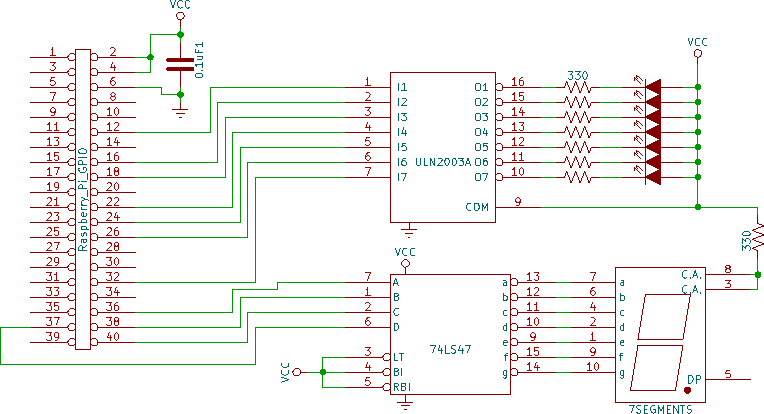
\includegraphics[width=0.9\columnwidth,height=8cm,keepaspectratio]{img/p03-diagram.pdf} %CHKTEX 8
	\caption{Diagrama de conexiones del circuito a alambrar}
	\label{fig:wiring-diagram} %CHKTEX 24
\end{figure}

\subsubsection{Subcircuito 1: leds en línea}.
Forme los siete leds en línea, cuidando de que todos tengan la misma orientación. A continuación, conecte el cátodo de cada LED a una resistencia de 300$\Omega$, y ésta a su vez a una salida libre del controlador ULN2003, de tal manera que el primer led de la fila esté conectado a la salida 1, el segundo a la salida 2, y así sucesivamente.

De manera similar, conecte las entradas 1 a 7 del ULN2003 a las salidas GPIO 18, 23, 24, 25, 8, 7, y 12 de la Raspberry Pi mediante el cable tipo listón (pines 12, 16, 18, 22, 24, 26 y 32).
La conexión de uno de los leds se conecte al GPIO12/PWM es importante, pues éste pin se utilizará para variar la intensidad del led más adelante.

Complete el alambrado del ULN2003 conectándolo a tierra, conectando el común de éste a VCC mediante el capacitor de 0.1$\mu$F. Finalmente, conecte el ánodo de todos los leds a VCC.%

\subsubsection{Subcircuito 2: Display de 7 segmentos}.
Comience conectando las salidas \emph{a} a \emph{g} del display del circuito controlador 74LS47 con los pines homónimos del display de siete segmentos.
A continuación, conecte el integrado a tierra y las terminales LT y RBI (pines 3 y 5) a VCC, dejando BI (pin 4) sin conectar tal como se muestra en la \Cref{fig:wiring-diagram}.
Como siguiente paso, conecte el ánodo común del display a VCC mediante una resistencia de 330$\Omega$.

A continuación conecte las entradas A, B, C, D a las salidas GPIO 16, 20, 21 y 26 respectivamente (pines 36, 38, 40 y 37 de la Raspberry Pi) mediante el cable tipo listón.

Finalmente, para terminar el alambrado, conecte el 74LS47 a VCC y tierra.

% %% %%%%%%%%%%%%%%%%%%%%%%%%%%%%%%%%%%%%%%%%%%%%%%%%%%%%%%%%%%%%%%%%%%
%
% Step 2
%
% %% %%%%%%%%%%%%%%%%%%%%%%%%%%%%%%%%%%%%%%%%%%%%%%%%%%%%%%%%%%%%%%%%%%
\subsection{Paso 2: Configuración y prueba del circuito}%
\label{sec:step2}
Antes de proceder, verifique conexiones con un multímetro en busca de corto circuitos. En particular verifique que exista una impedancia muy alta entre los pines 4 y 6 (VCC y tierra) del cable listón que conectará al GPIO de la Raspberry Pi.

Tras lo anterior, conecte VCC y tierra del circuito alambrado a un eliminador de corriente de 5V y cierre el circuito entre los pines 4 y 32 del cable listón. Si todo está alambrado correctamente, el último del de la fila deberá encender.

Ahora cierre el circuito entre los pines 4 y 37 del cable listón. Si todo está alambrado correctamente, el display de siete segmentos deberá mostrar un 1.

\paragraph{Importante:} Ninguno de los circuitos o resistencias debe calentarse.
Si alguno de los componentes emitiera calor, verifique las conexiones en busca de corto circuitos o reemplace los componentes dañados.

Verificadas las conexiones, instale los complementos de desarrollo del puerto de propósito general de la Raspberry Pi (deberían venir instalados por defecto).

\begin{Verbatim}[fontsize=\footnotesize]
$ sudo apt-get install python-rpi.gpio python3-rpi.gpio
\end{Verbatim}

% %% %%%%%%%%%%%%%%%%%%%%%%%%%%%%%%%%%%%%%%%%%%%%%%%%%%%%%%%%%%%%%%%%%%
%
% Step 3
%
% %% %%%%%%%%%%%%%%%%%%%%%%%%%%%%%%%%%%%%%%%%%%%%%%%%%%%%%%%%%%%%%%%%%%
\subsection{Paso 3: Led parpadeante}%
\label{sec:step3}
Con todas las conexiones probadas y verificadas, es seguro proceder al control de señales digitales utilizando el GPIO de la Raspberry Pi.

Inicie su Raspberry Pi y, ya sea mediante una terminal remota o directamente en ella, ejecute el siguiente código Python para hacer parpadear uno de los leds del circuito alambrado.

\medskip
\begin{lstlisting}
# Importa la librería de control del GPIO de la Raspberry Pi
import RPi.GPIO as GPIO
# Importa la función sleep del módulo time
from time import sleep

# Desactivar advertencias (warnings)
GPIO.setwarnings(False)
# Configurar la librería para usar el número de pin.
# Llame GPIO.setmode(GPIO.BCM) para usar el canal SOC definido por Broadcom
GPIO.setmode(GPIO.BOARD)
# Configurar el pin 32 como salida y habilitar en bajo
GPIO.setup(32, GPIO.OUT, initial=GPIO.LOW)

# El siguiente código hace parpadear el led
while True: # Bucle infinito
	sleep(0.5)                 # Espera 500ms
	GPIO.output(32, GPIO.HIGH) # Enciende el led
	sleep(0.5)                 # Espera 500ms
	GPIO.output(32, GPIO.LOW)  # Apaga el led
\end{lstlisting}
\medskip


% %% %%%%%%%%%%%%%%%%%%%%%%%%%%%%%%%%%%%%%%%%%%%%%%%%%%%%%%%%%%%%%%%%%%
%
% Step 4
%
% %% %%%%%%%%%%%%%%%%%%%%%%%%%%%%%%%%%%%%%%%%%%%%%%%%%%%%%%%%%%%%%%%%%%
\subsection{Paso 4: Led parpadeante con PWM}%
\label{sec:step4}
En lugar de utilizar tiempos de espera (mismos que consumen tiempo de procesamiento y energía), es posible hacer parpadear el led de manera mucho más precisa y rápida utilizando uno de los moduladores de ancho de pulso (en inglés \emph{Pulse Width Modulation} o \emph{PWM}) por hardware que incorpora la Raspberry Pi.

Ejecute el siguiente código Python para hacer parpadear uno de los leds del circuito alambrado.

\medskip
\begin{lstlisting}
# Importa la librería de control del GPIO de la Raspberry Pi
import RPi.GPIO as GPIO
# Importa la función sleep del módulo time
from time import sleep

# Desactivar advertencias (warnings)
GPIO.setwarnings(False)
# Configurar la librería para usar el número de pin.
GPIO.setmode(GPIO.BOARD)
# Configurar el pin 32 como salida y habilitar en bajo
GPIO.setup(32, GPIO.OUT, initial=GPIO.LOW)
# Inicializar el pin 32 como PWM a una frecuencia de 2Hz
pwm = GPIO.PWM(32, 1)

# El siguiente código hace parpadear el led
pwm.start(50)

flag = True
while flag:
	try:
		dutyCycle = int(input("Ingrese ciclo de trabajo: "))
		pwm.ChangeDutyCycle(dutyCycle)
	except:
		flag = False
		pwm.ChangeDutyCycle(0)
# Detiene el PWM
pwm.stop()
# Reinicia los puertos GPIO (cambian de salida a entrada)
GPIO.cleanup()
\end{lstlisting}


% %% %%%%%%%%%%%%%%%%%%%%%%%%%%%%%%%%%%%%%%%%%%%%%%%%%%%%%%%%%%%%%%%%%%
%
% Step 5
%
% %% %%%%%%%%%%%%%%%%%%%%%%%%%%%%%%%%%%%%%%%%%%%%%%%%%%%%%%%%%%%%%%%%%%
\subsection{Paso 5: Display de siete segmentos}%
\label{sec:step5}
El último ejemplo consiste en mostrar números en el display de siete segmentos.

Analice y ejecute el código mostrado a continuación.
\medskip
\begin{lstlisting}
# Importa la librería de control del GPIO de la Raspberry Pi
import RPi.GPIO as GPIO
# Importa la función sleep del módulo time
from time import sleep

# Desactivar advertencias (warnings)
GPIO.setwarnings(False)
# Configurar la librería para usar el número de pin.
GPIO.setmode(GPIO.BOARD)
# Configurar pines 36, 38, 40 y 37 como salida y habilitar en bajo
GPIO.setup(32, GPIO.OUT, initial=GPIO.LOW)
GPIO.setup(38, GPIO.OUT, initial=GPIO.LOW)
GPIO.setup(40, GPIO.OUT, initial=GPIO.LOW)
GPIO.setup(37, GPIO.OUT, initial=GPIO.LOW)

# Mapea bits a los pines de la GPIO
def bcd7(num):
	GPIO.output(32, GPIO.HIGH if num & 0x00000008 else GPIO.LOW )
	GPIO.output(38, GPIO.HIGH if num & 0x00000004 else GPIO.LOW )
	GPIO.output(40, GPIO.HIGH if num & 0x00000002 else GPIO.LOW )
	GPIO.output(37, GPIO.HIGH if num & 0x00000001 else GPIO.LOW )

flag = True
while flag:
	try:
		num = int(input("Ingrese número entero: "))
		bcd(num)
	except:
		flag = False
# Reinicia los puertos GPIO (cambian de salida a entrada)
GPIO.cleanup()
\end{lstlisting}

% %% %%%%%%%%%%%%%%%%%%%%%%%%%%%%%%%%%%%%%%%%%%%%%%%%%%%%%%%%%%%%%%%%%%
%
% Experiments
%
% %% %%%%%%%%%%%%%%%%%%%%%%%%%%%%%%%%%%%%%%%%%%%%%%%%%%%%%%%%%%%%%%%%%%
\section{Experimentos}%
\label{sec:experiments}

\begin{enumerate}
	\item{} [1pt] Modifique el código de la \cref{sec:step3} para todos los leds de la fila parpadeen.
	\item{} [1pt] Modifique el código de las \cref{sec:step3,sec:step5} para que los leds de la fila enciendan de manera continua en una marquesina de izquierda a derecha.
	\item{} [2pt] Modifique el código de las \cref{sec:step3,sec:step5} para que los leds de la fila enciendan de manera continua en una marquesina de derecha a izquierda con velocidad variable definida por el usuario.
	\item{} [1pt] Con base en las modificaciones anteriores, genere una marquesina que haga parecer que \enquote{la luz rebota} al llegar a las orillas (efecto ping-pong) con velocidad variable definida por el usuario.
	\item{} [3pt] Tomando como base el código de la \cref{sec:step4}, haga que uno de los leds encienda gradualmente a lo largo de un segundo hasta adquirir máxima potencia, permanezca encendido medio segundo, y después se apague gradualmente a lo largo de otro segundo.
\end{enumerate}

% %% %%%%%%%%%%%%%%%%%%%%%%%%%%%%%%%%%%%%%%%%%%%%%%%%%%%%%%%%%%%%%%%%%%
%
% Questionnaire
%
% %% %%%%%%%%%%%%%%%%%%%%%%%%%%%%%%%%%%%%%%%%%%%%%%%%%%%%%%%%%%%%%%%%%%
\section{Cuestionario}%
\label{sec:questionnaire}
\begin{enumerate}
	\item{} [0.5pt] Explique por qué usar corrimientos es la manera más eficiente de generar una marquesina.
	\item{} [0.5pt] Explique las ventajas o desventajas que tiene utilizar un modulador de ancho de pulso sobre tiempos de espera programados (\emph{delays}).
	\item{} [0.5pt] ¿Sería posible generar una marquesina circular utilizando el 74LS47 y el display de siete segmentos? Justifique su respuesta.
	\item{} [0.5pt] ¿Es posible configurar cualquier pin de la GPIO como PWM? Justifique su respuesta.
\end{enumerate}

\appendix

\cleardoublepage
\section{Programa Ejemplo: \texttt{blink.py}}%
\label{sec:appendix1}
\lstinputlisting[language=C,firstline=13]{src/blink.py}

\cleardoublepage
\section{Programa Ejemplo: \texttt{bcd.py}}%
\label{sec:appendix2}
\lstinputlisting[language=Python,firstline=14]{src/bcd.py}

\cleardoublepage
\section{Programa Ejemplo: \texttt{pwm.py}}%
\label{sec:appendix3}
\lstinputlisting[language=C,firstline=11]{src/pwm.py}

\cleardoublepage
\section{Programa Ejemplo: \texttt{pwm\_fast.py}}%
\label{sec:appendix3}
\lstinputlisting[language=C,firstline=11]{src/pwm_fast.py}%CHKTEX 25

\end{document}
